%!TEX root = ..\MainFile.tex
\chapter{КОМПЬЮТЕРНЫЕ МОДЕЛИ ГРУППОВОЙ ДИНАМИКИ}
\label{ch:ComputerModelsOfHords}

\epigraph{Позабыты~хлопоты,~остановлен~бег~- \\
Вкалывают роботы, а не человек.}{Ю. Энтин - ``Вкалывают роботы''}
Как было сказано в главе \ref{cha:NatureFlocking}, основной сложностью в исследовании процессов, происходящих в рое, является невозможность уследить сразу за всеми представителями. В первую очередь проблема заключается в высокой технической сложности гарантированно отличить одну особь от другой.

%!TEX root = ..\MainFile.tex
    \section{Основные модели} % (fold)
    \label{sec:CompModelsBasics}
    Моделированием групповых эффектов начали заниматься в 70е годы несколько групп ученых - биологов, физиков и специалистов по компьютерной графике. 
    \begin{figure}
        \centering
        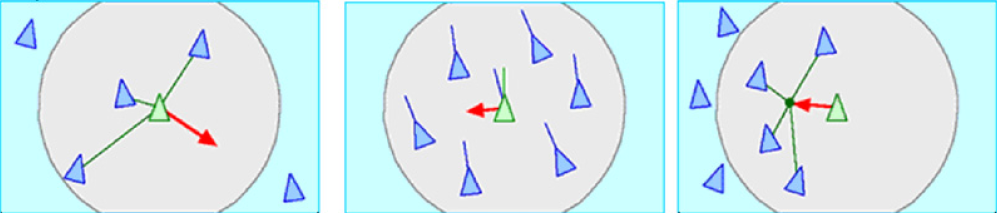
\includegraphics[width=\textwidth]{Images/Fig31_CollectiveMotion}
        \caption{Поведение, основное для модели Рейнольдса. (а) Разделение, с тем чтобы избежать чрезмерного скапливания боидов. (б) Выравнивание: боиды поворачивают в направлении средней скорости окружающих боидов. (в) Когезия: боиды смещаюстся в направлении центра масс окружения}
        \label{fig:ReynoldsModel}
    \end{figure}
    Первая широко известная модель была предложена Рейнольдсом~\cite{reynolds1987}. В его модели поведение обьектов (боидов) определялось из рассчета наилучшего визуального представления. Боиды могли демонстрировать три типа взаимодействия: избегание столкновений, следование в направлении ближайших боидов и стремление к центру масс стаи, см. рис. \ref{fig:ReynoldsModel}. 

    С тем, чтобы привнести в изучение групповых эффектов количественный подход, была предложена модель, широко известная сейчас как ``модель Вичека''~\cite{vicsek1995}. Поведение частиц в этой модели определяется следующими соотношениями:
    \begin{align}
    \label{eq:ViksecEquationsOfMotion}
        \vec{v}_i(t+1) &= v_0 \frac{{\langle \vec{v}_i(t) \rangle}_R}{|{\langle \vec{v_j}(t) \rangle}_R|} + perturbation \\
        \vec{x}_i(t+1) &= \vec{x}_i(t)+\vec{v}_i(t+1)
    \end{align}
    Здесь ${\langle \dots \rangle}_R$ обозначают усреднение (или суммирование) по всем частицам в радиусе $R$ вокруг $i$-й. Тогда $ \frac{{\langle \vec{v}_i(t) \rangle}_R}{|{\langle \vec{v_j}(t) \rangle}_R|}$ предоставляет нам единичный вектор в направлении средней скорости группы частиц. Такое выравнивающее правило не принимает во внимание характер взаимодействия, и потому модель может соответствовать когезии, взякости и тому подобному. Введение шума в модель может выполняться различными способами. В оригинальной работе было предложено следующее: поскольку единичный вектор однозначно соответствует углу, задающему направление, и скорость частиц также можно задавать в виде модуля скорости и единичного вектора направления, то тогда угол направления движения в момент времени $(t+1)$ получается следующим образом:
    \begin{equation}
        \vartheta_i (t+1) = \vartheta_i(t) + \Delta_i(t)
    \end{equation}
    где $\vartheta_i(t) = \arctan [{\frac{{\langle \vec{v}_i(t) \rangle}_R}{|{\langle \vec{v_j}(t) \rangle}_R|}}]$, и шум представлен $\Delta_i(t)$ - случайное число равновероятно выбранное из $[-\eta \pi,\eta \pi]$. Параметрами модели является плотность $\rho$, модуль скорости частиц $v_0$ и уровень шума, определяемый $\eta < 1$. Параметром порядка становится 
    $\varphi = 1/{N v_0} |{\sum\limits_{i=1}^n \vec{v_i}}|$, как определно в уравнени \ref{eq:OrederParam}.

    Несмотря на кажущуюся простоту этой модели, она демонстрирует богатый спектр свойств, характерных для систем, демонстрирующих групповую динамику. В первую очередь это, конечно же, фазовый переход к упорядоченному движению. Помимо этого, варьируя указанные выше параметры модели, удавалось получить различные паттерны, характерные для групповой динамики, а именно вращающиеся ``цепи'', ``ленты'', ``мельницы'', ``марширующие группы'' и другие.

    Интересным вопросом является род фазового перехода. В своей оригинальной работе Vicsek и соавторы показали, что наблюдается переход второго рода от разупорядоченного к упорядоченному движению. То есть, при переходе к термодинамическому пределу поведение параметра порядка недалеко от фазового перехода описывается
    \begin{equation}
        \varphi \sim [\eta_c(\rho)-\eta]^\beta
    \end{equation}
    \begin{equation}
        \varphi \sim [\rho-\rho_c(\eta)]^\delta
    \end{equation}
    Однако это было поставлена под вопрос Gr\'egoir and Chat\'e~\cite{gregoire2004}, что привело к серии работ адрессующих этот фундаментальный вопрос коллективного движения. В результате исследованиq Chat\'e и сооавторам~\cite{chate2008} удалось показать существование т.н. переходного режима, в котором происходит фазовый переход второго рода для любого значения скорости частиц.

    В общем, тип фазового перехода зависит от модуля скорости частиц и того, как шум вводится в систему. Для малых скоростей $v_0 < 0.5$, даже в пределе скорости $v_0 \to 0$ наблюдается фазовый переход второго рода. Для больших скоростей фазовый переход аналогичен фазовому переходу первого рода, косвенным свидетельством этого является формирование ``лент''.\cite{huepe2008}

    Существует две возможности привнести шум в систему: в виде случайного угла, на который поворачивается скорость частицы \textit{после} выравнивания с учетом направления движения окружения, и в виде случайного вектора, который добавляется ко всем частицам \textit{до} определения преимущественного направления движения. Первый вариант используется в модели Vicsek'a, в то время как второй вариант был предложен Gr\'egoir and Chat\'e~\cite{gregoire2004}. И как было показано численным експериментом~\cite{baglietto2008}, модель Вичека испытывает фазовый переход второго рода, в то время как при введении ``векторного'' шума возможно состояние при котором фазовый переход является переходом первого рода~\cite{aldana2009}.
% section CompModelsCollMot (end)


За годы прошедшие с момента создания модели Вичека, было предложено определенное количество моделей самодвижущихся частиц, воспроизводящих групповую динамику или отдельные характерные эффекты.

Можно выделить два типа такого рода моделей - в одних прямо вводится правило выравнивания частиц, а в других рассматривается опосредственное взаимодействие, к примеру, через столкновения или среду обитания. Однако, их обзор не входит в рамки данной работы, потому интересующимся рекомендуем обратиться к литературе, в особенности к ~\cite{vicsek2012}.